%!TEX root = ../crowd_hierarchies_kdd.tex

\section{Estimating the Gain of Queries}
\label{sec:gainestimators}
As discussed previously, crowd entity extraction queries are equivalent to retrieving samples from a population of items following an unknown popularity distribution. Deciding which query to issue is dictated by the estimated gain of each query, i.e., the expected number of newly extracted entities. Estimating the gain of a query requires reasoning about the population percentage covered by all entities extracted by previous queries as well as the expected number of unseen entities in the underlying population.

Recently, Trushkowsky et al. studied the problem of estimating the aforementioned quantities for queries of the form ``list one more entity'' - considering the entire population -  by drawing connections between the problem of crowdsourced entity extraction and that of species richness estimation~\cite{chao:1992}. The latter seeks to estimate the number of distinct species represented in an ecological community by obtaining samples from the underlying population. 

The techniques proposed by Trushkowsky et al.~\cite{trushkowsky:2013} extend an estimator proposed by Chao et al.~\cite{chao:1992} and are agnostic to the queries with exclude lists. Moreover, the original Chao estimator that they rely on, has been shown to exhibit negative biases~\cite{hwang:2010, shen:2003}, i.e., it underestimates the expected gain. Negative biases can severely impact entity extraction over large domains since nodes that contain entities that belong in the long tail of the popularity distribution may never be queried as they may be deemed to have zero population. In this section, we first review the existing methodology for estimating the gain of a query. Then we discuss how these estimators can be extended to consider an exclude list. Finally, we propose a new gain estimator for generalized queries $^vq(k,E)$ that exhibits lower biases, and thus, improved performance, in the presence of little information than previous techniques (see \Cref{sec:exps}).

\subsection{Previous Estimators}
\label{sec:prevest}
Consider a specific node $v \in \hierarchy$. Prior work only considers samples with replacement retrieved from the population associated with $v$ and does not consider an exclude list. Let $Q$ be the set of all existing samples retrieved by issuing queries at $v$ without an exclude list. These samples can be combined into a single sample, referred to as a {\em running sample}, corresponding to a multiset of size $n = \sum_{q \in Q} {\sf size}(q)$. Let $f_i$ denote the number of entities that appear $i$ times in this unified sample, and let $f_0$ denote the number of unseen entities from the population under consideration. Finally, let $C$ be the population coverage of the unified sample. i.e., the fraction of the population covered by the sample  $C = \frac{f_1 + f_2 + ..}{f_0 + f_1 + ...}$.

A new query $q^v(k,\emptyset)$ at node $v$ can be viewed as increasing the size of the unified sample by $k$. Prior work in crowdsourced entity extraction~\cite{trushkowsky:2013} used techniques from the species richness estimation literature to estimate the expected number of new entities extracted by a query $q^v(k,\emptyset)$ that does not use an exclude list. Originally, Shen et al.~\cite{shen:2003}, proposed an estimator for the number of new species $\hat{N}_{Shen}$ that would be found in an increased sample of size $k$. The approach assumes that unobserved entities have equal relative popularity. An estimate of the unique elements found in an increased sample of size $k$ is given by:

\begin{equation}
\label{eq:shen}
\hat{N}_{Shen} = f_0\left( 1 - \left(1 - \frac{1 - C}{f_0}\right)^k\right)
\end{equation}
\vspace{5pt}

Considering the scenario of crowdsourced entity extraction, the second term of Shen's formula corresponds to the probability that at least one unseen entity will be present in a query asking for $k$ more entities. Thus, multiplying this quantity with the number of unseen entities $f_0$ corresponds to the expected number of unseen entities present in the result of a new query $q^v(k,\emptyset)$.

The quantities $f_0$ and $C$ are unknown and thus need to be estimated for the population corresponding to node $v$ considering the observed entities in the running sample associated with $v$. The coverage can be estimated by considering the Good-Turing estimator $\hat{C} = 1 - \frac{f_1}{n}$ for the existing retrieved sample. On the other hand, multiple estimators have been proposed for estimating the number of unseen entities $f_0$. Trushkowsky et al.~\cite{trushkowsky:2013} proposed a variation of an estimator introduced by Chao et al.~\cite{chao:1992} to estimate $f_0$. Nevertheless, the authors argue that the original estimator proposed by Chao performs similarly with their approach when estimating the gain of an additional query. 

The original Chao estimator relies on the sample coverage $C$ to estimate the number of unseen items. Moreover, it attempts to characterize and incorporate the skew of the underlying popularity distribution by utilizing the information captured by the available $f_i$ counts~\cite{chao:1992}. Recently, Hwang et al.~\cite{hwang:2010} proposed an alternative estimator for $f_0$ that is more robust in the presence of little information and utilizes a regression technique that exploits the information available in all $f_i$ counts.  

Until now we focused on samples obtained by directly querying node $v$ and without considering an exclude list. Next, we discuss how one can estimate the return of a query $q^v(k,E)$ by considering all observed entities associated with node $v$, potential negative answers, and discuss how the previous estimators can be used in the presence of an exclude list $E$.

\subsection{Indirect Sampling}
\label{sec:indirectsampling}
Given a structured domain, the extracted entities for a node $v$ can be obtained either by querying node $v$ directly or by indirect information flowing to $v$ by queries at other nodes connected to $v$. We refer to the latter case as {\em indirect sampling}. Eventually, we have two different kinds of samples: (i) those that were extracted by considering the {\bf entire population} corresponding to node $v$ (ii) and those that extracted by sampling {\bf only a part of the population} corresponding to $v$. 
\begin{figure}
	\begin{center}
	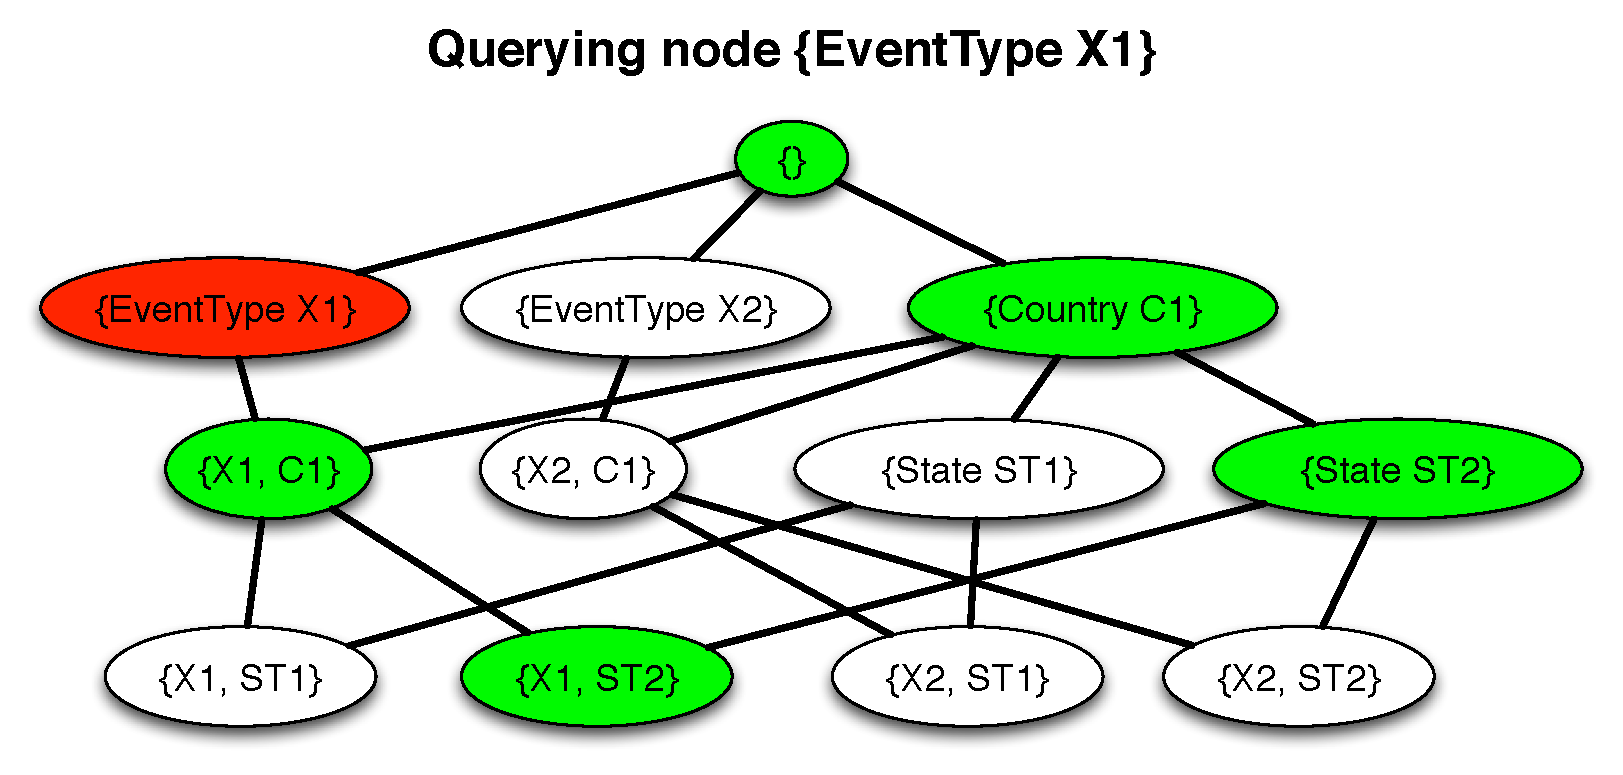
\includegraphics[clip,scale=0.3]{figs/exampleQuery.eps}	
	\caption{An example query that extracts an entity sample from the red node. The nodes marked with green correspond to the nodes for which indirect entity samples are retrieved.}
	\label{fig:query}
	\vspace{-20pt}
	\end{center}
\end{figure}
We use an example considering the poset in \Cref{fig:eventslattice}, to illustrate these two cases. The example is shown in \Cref{fig:query}. Assume a query $q(k,0)$ issued against node \{EventType X1\}. Assume that the query result contains entities that correspond only to node \{X1,ST2\}. The green nodes in \Cref{fig:query} are nodes for which samples are obtained indirectly without querying them. Notice, that all these nodes are ancestors of \{X1,ST2\}. We have:
\squishlist
\item The samples corresponding to nodes \{X1, C1\} and \{X1,ST2\} were obtained by considering their {\em entire population}. The reason is that node \{EventType X1\} is an ancestor of both and the entity population corresponding to it fully contains the populations of both \{X1,C1\} and \{X1,ST1\}. 
\item The samples corresponding to nodes \{ \}, \{Country C1\} and \{State ST2\} were obtained by considering only part of their population. The reason is that the population of node \{EventType X1\} does not fully contain the populations of these nodes. 
\squishend

Samples belonging to both types need to be considered when estimating the gain of a query at a node in $v \in \hierarchy$. To address this issue we merge the extracted entities for each node in $\hierarchy$ into a single sample and treat the unified sample as being extracted from the entire underlying population of the node. As we discuss later in \Cref{sec:solving} we develop querying strategies that traverse the poset $\hierarchy$ in a top-down approach, hence, the number of samples belonging in the first category, i.e., samples retrieved considering the entire population of a node, dominates the number of samples retrieved by considering only part of a node's population. Moreover, it has been shown by Hortal et al.~\cite{hortal2006evaluating} that several of the existing techniques used to estimate the gain of a query (see \Cref{sec:prevest}) are insensitive to differences in the way samples are aggregated.

\subsection{Exclude Lists and Negative Answers}
\label{sec:excludelist}
A query $q^v(k, E)$ with $E \ne \emptyset$ issued at node $v \in H_D$ effectively limits the sampling to a restricted subset of the entity population corresponding to node $v$. To estimate the expected return of such a query, we need to update the estimates $\hat{f}_0$ and $\hat{C}$ before applying \Cref{eq:shen}, by removing the entities in $E$ from the running sample for node $v$ and updating the frequency counts $f_i$ and sample size $n$. This approach requires that the exclude list is known in advance. We discuss how we construct an exclude list in \Cref{sec:heuristic}.

Finally, we consider the effect of {\em negative answers} on estimating the gain of future queries. It is possible to issue a query at a specific node $v \in \hierarchy$ and receive no entities, i.e., we receive a negative answer. This is an indication that the underlying entity population of $v$ is empty. In such a scenario, we assign the expected gain of future queries at $v$ and all its descendants to zero. Another type of negative answer corresponds to issuing a query at an ancestor node $u$ of $v$ and receiving no entities for $v$. In this case, we do not update our estimates for node $u$ as entities from other descendants of $u$ may be more popular than entities associated with $u$.

\subsection{Direct Gain Estimation}
\label{sec:newestim}
The techniques reviewed in \Cref{sec:prevest} result in negative bias when the number of observed entities from a population represents only a {\em small fraction} of the entire population~\cite{hwang:2010, shen:2003}. This holds for the large and sparse domains we consider in this paper. To address this problem, Hwang and Shen~\cite{hwang:2010} proposed a regression based technique to estimate $f_0$ and show that it results in smaller biases. However, estimating the total gain of a query requires coupling this new estimator with \Cref{eq:shen}, thus, it may still exhibit negative bias. To eliminate negative bias, we propose a direct estimator for the gain of generalized queries $q(k,E)$ without using \Cref{eq:shen}. We build upon the techniques in~\cite{hwang:2010} and use a regression based technique that captures the structural properties of the expected gain function. The proofs for the results below can be found in the Appendix.

Let $S$ denote the total number of entities in the population under consideration and $p_i$ the abundance probability (i.e., popularity) of entity $i$. Given a sample of size $n$ from the population, define $K(n)$ to be $K(n) = \frac{\sum_{i=1}^S (1-p_i)^n}{\sum_{i=1}^S p_i(1-p_i)^{n-1}}$. First, we focus on queries without an exclude list. Later we relax this and discuss queries with exclude lists. We have the following theorem on query gain:

\vspace{-5pt}\begin{theorem}
\label{newgain}
Given a node $v \in \hierarchy$ and a corresponding entity sample of size $n$, let $f_1$ and $f_2$ denote the number of entities that appear exactly once (i.e., singletons) and exactly twice respectively. Let $G$ denote the number of new items retrieved by a query $q(m,\emptyset)$. We have that:

\vspace{-10pt}\begin{equation}
\label{eq:dirgain}
G = \frac{1}{(1 + \frac{K^{\prime}}{n+m})}(K\frac{f_1}{n} - K^{\prime}\frac{f_1(1-\frac{1}{n}2\frac{f_2}{f_1})^m}{n+m})
\end{equation}
where $K = K(n)$ and $K^{\prime} = K(n+m)$.
\end{theorem}
\iftr
\begin{proof}
To derive the new estimator we make used of the generalized jackknife procedure for species richness estimation~\cite{heltshe1983estimating}. Given two (biased) estimators of $S$, say $\hat{S}_1$ and $\hat{S}_2$, let $R$ be the ratio of their biases:
\begin{equation}
R = \frac{E(\hat{S}_1) - S}{E(\hat{S}_2) - S}
\end{equation}
By the generalized jackknife procedure, we can completely eliminate the bias resulting from either $\hat{S}_1$ or $\hat{S}_2$ via
\begin{equation}
S = G(\hat{S}_1, \hat{S}_2) = \frac{\hat{S}_1 - R\hat{S}_2}{1 - R}
\label{eq:jknife}
\end{equation}
provided the ratio of biases $R$ is known. However, $R$ is unknown and needs to be estimated. 

Let $D_n$ denote the number of unique entities in a unified sample of size $n$. We consider the following two biased estimators of $S$: $\hat{S_1} = D_n$ and $\hat{S}_2 = \sum_{j=1}^n D_{n-1}(j)/n = D_n - f_1/n$ where $D_{n-1}(j)$ is the number of species discovered with the $j$th observation removed from the original sample. Replacing these estimators in \Cref{eq:jknife} gives us:
\begin{equation}
S = D_n +\frac{R}{1-R}\frac{f_1}{n}
\end{equation}
Similarly, for a sample of increased size $n+m$ we have:
\begin{equation}
S = D_{n+m} +\frac{R^{\prime}}{1-R^{\prime}}\frac{f^{\prime}_1}{n+m}
\end{equation}
where $R^{\prime}$ is the ratio of the biases and $f^{\prime}_1$ the number of singleton entities for the increased sample. Let $K = \frac{R}{1-R}$ and $K^{\prime} = \frac{R^{\prime}}{1-R^{\prime}}$. Taking the difference of the previous two equations we have:
\begin{equation}
D_{n+m} - D_{n} = K\frac{f_1}{n} - K^{\prime}\frac{f^{\prime}_1}{n+m}
\end{equation}
Therefore, we have:
\begin{equation}
\label{eq:new}
G = K\frac{f_1}{n} - K^{\prime}\frac{f^{\prime}_1}{n+m}
\end{equation}
We need to estimate $K$, $K^{\prime}$ and $f^{\prime}_1$. We start with $f^{\prime}_1$, which denotes the number of singleton entities in the increased sample of size $n+m$. Notice, that $f^{\prime}_1$ is not known since we have not obtained the increased sample yet, so we need to express it in terms of $f_1$, i.e., the number of singletons, in the running sample of size $n$. We have:
\begin{equation}
f^{\prime}_1 = G + f_1 - f_1^c
\end{equation}
where $f_1^c$ denotes the number of old singleton entities from the sample of size $n$ that appeared in the additional query of size $m$. Let $E_1$ denote the set of singleton entities in the old sample of size $n$. We approximate $f_1^c$ by its expected value:
\begin{equation}
\hat{f}_1^c = \sum_{e \in E_1} \Pr[\mbox{e appears in query of size $m$}]
\end{equation}
We compute the probability of an old singleton entity appearing in an additional query as follows. Let $p_e$ denote the popularity of entity $e$. As described before, an additional query of size $m$ corresponds to taking a sample of size $m$ from the underlying entity population without replacement. However, $m$ is significantly smaller compared to the size of the underlying population, thus, we can consider a that taking a sample of size $m$ corresponds to taking a sample {\em with replacement}. Following this we have that:
\begin{equation}
\Pr[\mbox{e appears in query of size $m$}] = 1 - (1-p_e)^m
\end{equation}
Following a standard approach in the species estimation literature we assume that the popularity of retrieving a singleton entity again is the same for all singleton entities. This popularity can be computed using the corresponding Good-Turing estimator considering the running sample. We have:
\begin{equation}
\forall e \in E_1, p_e = p_1 = \hat{\theta}(1) = \frac{1}{n}2\frac{f_2}{f_1}
\end{equation}
where $f_2$ is the number of entities that appear twice in the sample and $f_1$ is the number of singletons. 
Eventually we have that:
\begin{equation}
\hat{f}_1^c = f_1(1 - (1-p_1)^m)
\end{equation}
and
\begin{equation}
f^{\prime}_1 = G + f_1(1-p_1)^m
\end{equation}
Replacing the last equation in \Cref{eq:new} we have:
\begin{align}
&G = K\frac{f_1}{n} - K^{\prime}\frac{G + f_1(1-p_1)^m}{n+m} \nonumber \\
&G = K\frac{f_1}{n} - K^{\prime}\frac{G}{n+m} - K^{\prime}\frac{f_1(1- P)}{n+m} \nonumber \\
&G(1 + \frac{K^{\prime}}{n+m}) = K\frac{f_1}{n} - K^{\prime}\frac{f_1(1- P)}{n+m} \nonumber \\
&G = \frac{1}{(1 + \frac{K^{\prime}}{n+m})}(K\frac{f_1}{n} - K^{\prime}\frac{f_1(1-p_1)^m}{n+m}) \nonumber
\end{align}
\end{proof}
\fi
All quantities apart from $K$ and $K^{\prime}$ in \Cref{eq:dirgain} are known. The value of $K$ can be estimated using the regression approach introduced by Hwang and Shen~\cite{hwang:2010}. \iftr From the Cauchy-Schwarz inequality we have that:
\begin{equation}
K = \frac{\sum_{i=1}^S (1-p_i)^n}{\sum_{i=1}^S p_i(1-p_i)^{n-1}} \geq \frac{(n-1)f_1}{2f_2}
\end{equation}
This can be generalized to:
\begin{equation}
K=\frac{nf_0}{f_1} \geq \frac{(n-1)f_1}{2f_2} \geq \frac{(n-2)f_2}{3f_3} \geq \dots
\end{equation}
Let $g(i) = \frac{(n-i)f_i}{(i+1)f_{i+1}}$. From the above we have that the function $g(x)$ is a smooth monotone function for all $x \geq 0$. Moreover, let $y_i$ denote a realization of $g(i)$ mixed with a random error. Hwang and Shen how one can use an exponential regression model to estimate $K$. The proposed model corresponds to:
\begin{equation}
y_i = \beta_0\exp(\beta_1i^{\beta_2}) + \epsilon_i
\end{equation}
where $i = 1, \dots, n-1$, $\beta_0 > 0$, $\beta_1 < 0$, $\beta_2 >0$ and $\epsilon_i$ denotes random errors. It follows that $K = \beta_0$. \fi
To estimate the value of $K^{\prime}$ for an increased sample of size $n+m$, we first show that $K$ increases monotonically as the size of the running sample increases. 

\begin{lemma}
\label{monotonicity}
The function $K(n) = \frac{\sum_{i=1}^S (1-p_i)^n}{\sum_{i=1}^S p_i(1-p_i)^{n-1}}$ increases monotonically, i.e., $K(n+m) \geq K(n), \forall n,m > 0$.
\end{lemma}
\iftr
\begin{proof}
In the remainder of the proof we will denote $K(n+m)$ as $K^{\prime}$. By definition we have that $K = \frac{\sum_{i=1}^S (1-p_i)^n}{\sum_{i=1}^S p_i(1-p_i)^{n-1}}$ and $K^{\prime} = \frac{\sum_{i=1}^S (1-p_i)^{n+m}}{\sum_{i=1}^S p_i(1-p_i)^{n+m-1}}$. We want to show that:

{\small
\begin{align}
&\frac{\sum_{i=1}^S (1-p_i)^{n+m}}{\sum_{i=1}^S p_i(1-p_i)^{n+m-1}} \geq \frac{\sum_{i=1}^S (1-p_i)^n}{\sum_{i=1}^S p_i(1-p_i)^{n-1}} \nonumber \\
&\sum_{i=1}^S (1-p_i)^{n+m}\sum_{j=1}^S p_j(1-p_j)^{n-1} \geq \sum_{i=1}^S p_i(1-p_i)^{n+m-1}\sum_{j=1}^S (1-p_j)^n\nonumber \\
&\sum_{i,j:i\prec j}[(1-p_i)^{n+m}p_j(1-p_j)^{n-1} - p_i(1-p_i)^{n+m-1}(1-p_j)^n + \nonumber \\
& + (1-p_j)^{n+m}p_i(1-p_i)^{n-1} - p_j(1-p_j)^{n+m-1}(1-p_i)^n] \geq 0 \nonumber \\
%&\sum_{i,j:i\prec j}[(1-p_i)^{n}(1-p_j)^{n-1}p_j((1-p_i)^{m} - (1-p_j)^{m})  + \nonumber \\
%& - (1-p_j)^{n}p_i(1-p_i)^{n-1}((1-p_i)^{m} - (1-p_j)^{m}) \geq 0 \nonumber \\
&\sum_{i,j:i\prec j}[(1-p_i)^{n-1}(1-p_j)^{n-1}(p_j-p_i)((1-p_i)^{m} - (1-p_j)^{m}) \geq 0
\end{align}}

But the last inequality always holds since each term of the summation is positive. In particular, if $p_j \geq p_i$ then
also $1-p_i \geq 1-p_j$ and if $p_j \leq p_i$ then $1-p_i \leq 1-p_j$.
\end{proof}
\fi
Given the monotonicity of function $K$, we model $K$ as a generalized logistic function of the form $K(x) = \frac{A}{1+exp(-G(x-D))}$. As we observe samples of different sizes for different queries we estimate $K$ as described above and therefore we observe different realizations of $f(\cdot)$. Thus, we can learn the parameters of $f$ and use it to estimate $K^{\prime}$. In the presence of an exclude list of size $l$ we follow the approach described in \Cref{sec:excludelist} to update the quantities $f_i$ and $n$ used in the analysis above. 

%\subsection{Negative Answers and Gain Estimation}
%\label{sec:neg}
%Next, we study the effect of {\em negative answers} on estimating the gain of future queries. It is possible to issue a query at a specific node $v \in \hierarchy$ and receive no entities, i.e., we receive a negative answer. This is an indication that the underlying entity population of $v$ is empty. In such a scenario, we assign the expected gain of future queries at $v$ and all its descendants to zero. 
%
%Another type of negative answer corresponds to the scenario where we issue a query at an ancestor node $u$ of $v$ and receive no entities associated with $v$ but received some entities for $u$. Notice, that in this case, we do not have enough information to update our estimates for node $u$. The reason is that due to the restricted query size entities from other descendants of $u$ may be more popular with respect to the popularity distribution of $u$.